\documentclass{beamer}
\usepackage{xcolor}
\usepackage{natbib} % package to organize literature
\usepackage{multicol}
\usepackage{booktabs}
\usepackage{wasysym} % additional symbols
\usepackage{graphicx} % to include graphics, gifs
\usepackage{color} % add colored text
\usepackage{lmodern} % to fix font size error, might be problematic with math symbols
\usepackage{array}

\usetheme{Frankfurt}
\usecolortheme{beaver}
\setbeamertemplate{footline}
{
  \leavevmode%
  \hbox{%
  \begin{beamercolorbox}[wd=.3\paperwidth,ht=2.25ex,dp=1ex,center]{author in head/foot}%
    \usebeamerfont{author in head/foot}\insertshortauthor \hspace{1em} (\insertshortinstitute)
  \end{beamercolorbox}%
  \begin{beamercolorbox}[wd=.4\paperwidth,ht=2.25ex,dp=1ex,center]{title in head/foot}%
    \usebeamerfont{title in head/foot}\insertshorttitle
  \end{beamercolorbox}%
  \begin{beamercolorbox}[wd=.3\paperwidth,ht=2.25ex,dp=1ex,right]{author in head/foot}%
    \usebeamerfont{author in head/foot}\insertdate \hspace{2em}
    \insertframenumber{} / \inserttotalframenumber\hspace*{1em}
  \end{beamercolorbox}}%
  \vskip0pt%
}
%\definecolor{beamer@sbred}{rgb}{0.65,0.15,0.18}
\definecolor{beamer@sbred}{rgb}{0.22,0.22,0.66}
\setbeamercolor{title}{fg=beamer@sbred,bg=black!5}
\setbeamercolor{structure}{fg=beamer@sbred}
\setbeamercolor{frametitle}{fg=beamer@sbred}
\setbeamercolor{palette primary}{fg=beamer@sbred,bg=black!10}
\setbeamercolor{palette secondary}{fg=beamer@sbred}
\setbeamercolor{palette tertiary}{bg=beamer@sbred}
\setbeamercolor{palette quaternary}{fg=white,bg=beamer@sbred}
\setbeamertemplate{itemize items}[default]
\setbeamertemplate{enumerate items}[default]
\setbeamersize{text margin left=1em,text margin right=1em}
\DeclareTextFontCommand{\emph}{\color{beamer@sbred}}

\setbeamercolor*{block title example}{fg= white, bg= beamer@sbred!90}
\setbeamercolor*{block body example}{fg= black, bg= beamer@sbred!10}

\author[Patrick Kraft]{Patrick Kraft}
\institute[Stony Brook]{73rd MPSA Conference}
\title[Moral Foundations of Political Reasoning]{Moral Foundations of Political Reasoning \\ {\small Investigating the Moral Underpinnings of Political Judgment}}
\date{April 16\textsuperscript{th}, 2015}
\titlegraphic{\includegraphics[width=4cm]{/data/Copy/1-src/logos/logo_bk.pdf}}

\begin{document}
\frame{\titlepage}
%\footnotesize


\section{Introduction}
\subsection{}
\begin{frame}%[allowframbreaks]
\frametitle{Open-ended survey response in 2012 ANES}
\begin{exampleblock}{Is there anything in particular about [Candidate] that might make you want to vote for him? What is that?}
  \begin{center}
    \textit{``I think he represents a far more healthy vizsion for the country on a lot of levels, economically, environmentally, the vision he represents for the future of the country is much more in line with the country I hope to leave for my grandchildren, socially - protecting the rights of individuals, specifically the rights of women and individuals, the right to choose, picking a Supreme Court Justice and developing a tax system that is fair to everyone. [...]''}
  \end{center}
\end{exampleblock}
\end{frame}

\subsection{}
\begin{frame}%[allowframbreaks]
  \frametitle{Questions}
  \begin{itemize}
    \item Do individuals rely on \emph{moral foundations} when evaluating political \emph{parties} and \emph{candidates} \citep{haidt2008moral}?
    \item Are there systematic differences between \emph{liberals} and \emph{conservatives} \citep{haidt2007morality,graham2009liberals}?
    \item Are moral values \emph{determinants} of political thinking, or only a \emph{rhetorical device} that citizens \emph{learn} to bolster their political views?
  \end{itemize}
\end{frame}

\section{}
\subsection{}
\begin{frame}%[allowframbreaks]
  \frametitle{Hypotheses}
  \begin{enumerate}
    \item \emph{Liberals} are more likely to emphasize moral foundations of \emph{harm/care} and \emph{fairness/reciprocity} than conservatives when evaluating political parties and candidates. On the other hand, \emph{conservatives} are more likely to emphasize moral foundations of \emph{ingroup/loyalty}, \emph{authority/respect}, and \emph{purity/sanctity} than liberals.
    \item Individuals who have more experience and are more engaged in the political system (i.e. with higher \emph{political sophistication}, high \emph{media exposure}, frequent \emph{political discussions}, prior \emph{participation}) are more likely to emphasize moral foundations when evaluating political parties and candidates.
  \end{enumerate}
\end{frame}

\section{Empirical Analyses}
\subsection{}
\begin{frame}%[allowframbreaks]
  \frametitle{Overview}
  \begin{itemize}
    \item 2012 + 2008 American National Election Study (pre-election)
    \item Computer assisted face-to-face interviews (+ internet panel)
    \item Major dependent variable: \emph{open-ended questions} where respondents were asked what they \emph{liked} and \emph{disliked} about the parties and candidates
    \item Moral Foundations \emph{dictionary} proposed by \citep{graham2009liberals} to look for \emph{signal} words.
    \item Model individual response patterns for each of the moral foundations
  \end{itemize}
\end{frame}

\subsection{}
\begin{frame}%[allowframbreaks]
  \frametitle{Analyzing Open-Ended Survey Responses}
\begin{exampleblock}{Is there anything in particular about [Candidate] that might make you want to vote for him? What is that?}
  \begin{center}
    \textit{``I think he represents a far more healthy \underline{vision} for the country on a lot of levels, economically, environmentally, the vision he represents for the future of the country is much more in line with the country I hope to leave for my grandchildren, socially - {\color{blue}protecting} the {\color{green}rights} of {\color{red}individuals}, specifically the {\color{green}rights} of women and {\color{red}individuals}, the right to choose, picking a Supreme Court {\color{green}Justice} and developing a tax system that is {\color{green}fair} to everyone. [...]''}
  \end{center}
\end{exampleblock}
  \begin{itemize}
  \item \emph{\textit{Moral Foundations}}: {\color{blue}Harm}, {\color{green}Fairness}, {\color{red}Ingroup}
  \end{itemize}
\end{frame}

\subsection{}
\begin{frame}%[allowframbreaks]
  \frametitle{Descriptive Results}
  \begin{figure}[ht]\centering
    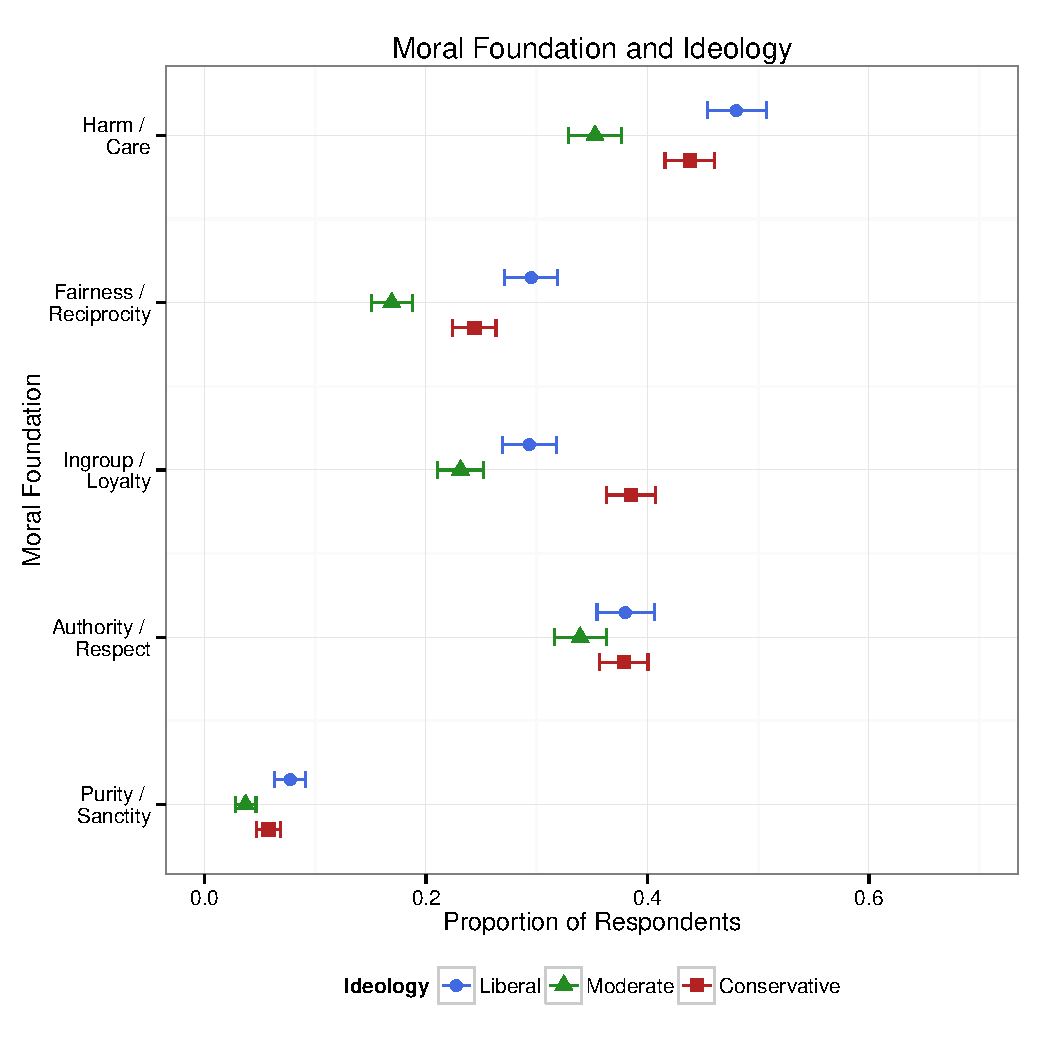
\includegraphics[height=.9\textheight]{../calc/fig/p1_mft_ideol}
  \end{figure}
\end{frame}

\subsection{}
\begin{frame}%[allowframbreaks]
  \frametitle{Predicting References to Moral Foundations}
  \begin{figure}[ht]\centering
    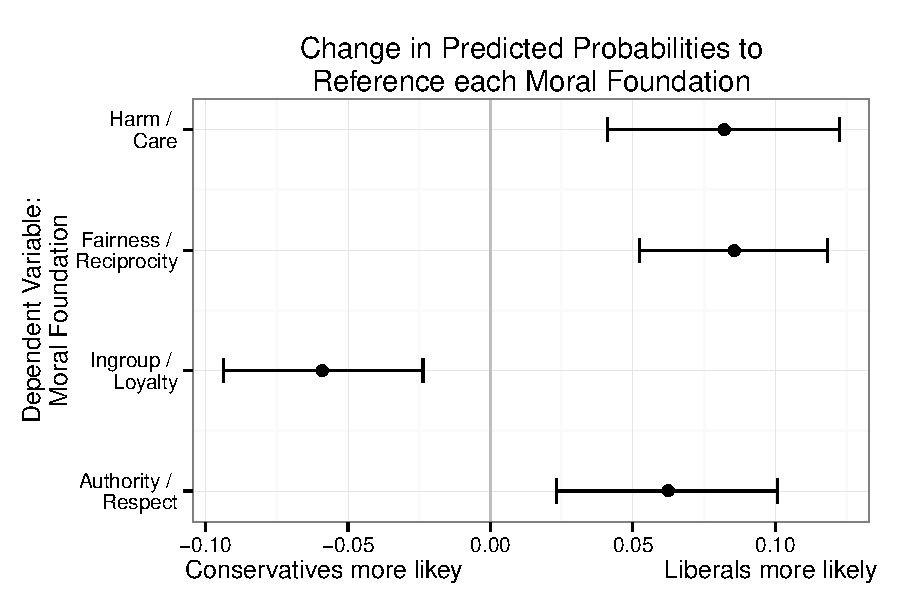
\includegraphics[height=.9\textheight]{../calc/fig/m1_mft}
  \end{figure}
\end{frame}

\subsection{}
\begin{frame}%[allowframbreaks]
  \frametitle{Moral Reasoning as a Political Learning Process}
  \begin{figure}[ht]\centering
    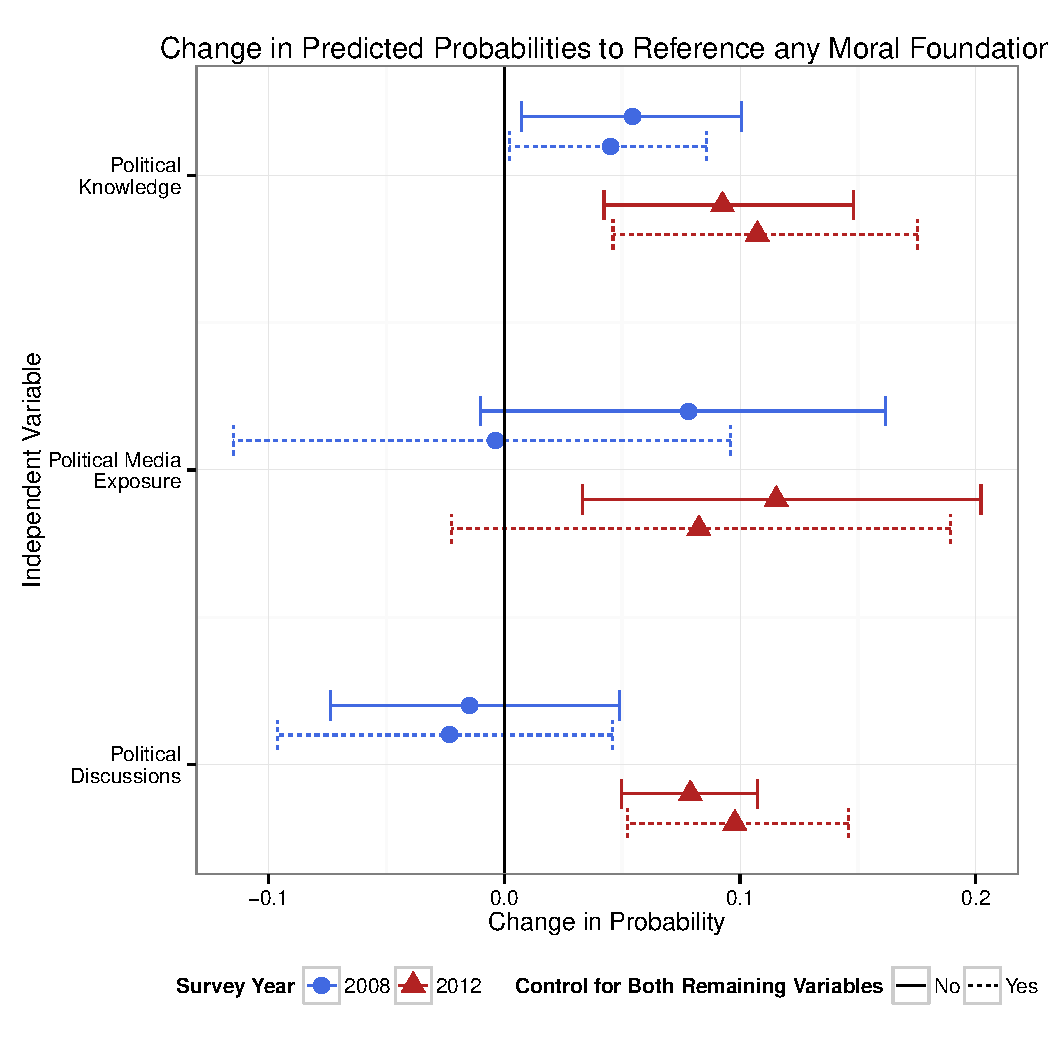
\includegraphics[height=.9\textheight]{../calc/fig/m3_learn}
  \end{figure}
\end{frame}

\section{Conclusion}
\subsection{}
\begin{frame}%[allowframbreaks]
  \frametitle{Conclusion}
  \begin{itemize}
\item Open-ended survey responses provide a useful \emph{unobtrusive measure} to investigate the relationship between moral considerations and political reasoning
\item \emph{Liberals} and \emph{conservatives} differ in their emphasis on moral dimensions
\item Differences not always consistent with \emph{Moral Foundations Theory} (fuzzy measurement etc.)
\item Political \emph{learning} process
\item \emph{Further developments}:
    \begin{itemize}
     \item Revise dictionary
     \item Differentiate between rejection/approval of moral foundations, in-party/out-party, candidate vs. party, etc.
     \item Development over longer time period, effect of polarization
     \item Structural topic models \citep{roberts2014structural}
     \item Experimental designs
    \end{itemize}
  \end{itemize}
\end{frame}

\subsection{}
\begin{frame}%[allowframbreaks]
\frametitle{Open-ended survey response in 2012 ANES}
\begin{exampleblock}{Is there anything in particular about [Party] that might make you want to vote against him? What is that?}
  \begin{center}
    \textit{``The party is run by Satan - it's filled with liars, cheaters, murderers, the sexually immoral, etc. Should you reject God in life, I am sure you'll be joined alongside in hell by most [members of party], with all of you fighting to be lord of that domain also.''}
  \end{center}
\end{exampleblock}
\end{frame}



\section{Appendix}
\subsection{}
\begin{frame}%[allowframbreaks]
  \frametitle{Moral Foundations Dictionary \citep[c.f.][]{graham2009liberals}}
  \begin{tiny}
    \begin{itemize}
      \item \emph{Harm:} safe*, peace*, compassion*, empath*, sympath*, care, caring, protect*, shield, shelter, amity, secur*, benefit*, defen*, guard*, preserve, harm*, suffer*, war, wars, warl*, warring, fight*, violen*, hurt*, kill, kills, killer*, killed, killing, endanger*, cruel*, brutal*, abuse*, damag*, ruin*, ravage, detriment*, crush*, attack*, annihilate*, destroy, stomp, abandon*, spurn, impair, exploit, exploits, exploited, exploiting, wound*

      \item \emph{Fairness:} fair, fairly, fairness, fair*, fairmind*, fairplay, equal*, justice, justness, justifi*, reciproc*, impartial*, egalitar*, rights, equity, evenness, equivalent, unbias*, tolerant, equable, balance*, homologous, unprejudice*, reasonable, constant, honest*, unfair*, unequal*, bias*, unjust*, injust*, bigot*, discriminat*, disproportion*, inequitable, prejud*, dishonest, unscrupulous, dissociate, preference, favoritism, segregat*, exclusion, exclud*

      \item \emph{Ingroup:} together, nation*, homeland*, family, families, familial, group, loyal*, patriot*, communal, commune*, communit*, communis*, comrad*, cadre, collectiv*, joint, unison, unite*, fellow*, guild, solidarity, devot*, member, cliqu*, cohort, ally, insider, foreign*, enem*, betray*, treason*, traitor*, treacher*, disloyal*, individual*, apostasy, apostate, deserted, deserter*, deserting, deceiv*, jilt*, imposter, miscreant, spy, sequester, renegade, terroris*, immigra*

      \item \emph{Authority:} obey*, obedien*, duty, law, lawful*, legal*, duti*, honor*, respect, respectful*, respected, respects, order*, father*, mother, motherl*, mothering, mothers, tradition*, hierarch*, authorit*, permit, permission, status*, rank*, leader*, class, bourgeoisie, caste*, position, complian*, command, supremacy, control, submi*, allegian*, serve, abide, defere*, defer, revere*, venerat*, comply, defian*, rebel*, dissent*, subver*, disrespect*, disobe*, sediti*, agitat*, insubordinat*, illegal*, lawless*, insurgent, mutinous, defy*, dissident, unfaithful, alienate, defector, heretic*, nonconformist, oppose, protest, refuse, denounce, remonstrate, riot*, obstruct

      \item \emph{Purity:} piety, pious, purity, pure*, clean*, steril*, sacred*, chast*, holy, holiness, saint*, wholesome*, celiba*, abstention, virgin, virgins, virginity, virginal, austerity, integrity, modesty, abstinen*, abstemiousness, upright, limpid, unadulterated, maiden, virtuous, refined, intemperate, decen*, immaculate, innocent, pristine, humble, disgust*, deprav*, disease*, unclean*, contagio*, indecen*, sin, sinful*, sinner*, sins, sinned, sinning, slut*, whore, dirt*, impiety, impious, profan*, gross, repuls*, sick*, promiscu*, lewd*, adulter*, debauche*, defile*, tramp, prostitut*, unchaste, wanton, profligate, filth*, trashy, obscen*, lax, taint*, stain*, tarnish*, debase*, desecrat*, wicked*, blemish, exploitat*, pervert, wretched*
    \end{itemize}
  \end{tiny}
\end{frame}

\subsection{}
\begin{frame}%[allowframbreaks]
\frametitle{Missing Open-ended Responses}
% latex table generated in R 3.2.2 by xtable 1.7-4 package
% Wed Sep 16 10:56:58 2015
\begin{table}[ht]
\centering
\begin{tabular}{lcc}
  \hline
 & N & Percent \\ 
  \hline
Spanish Interview (2008) & 94 & 4.05 \\ 
  Spanish Interview (2012) & 228 & 3.86 \\ 
  No Responses (Overall, 2008) & 158 & 7.09 \\ 
  No Responses (Overall, 2012) & 392 & 6.89 \\ 
  No Responses (Candidate Evaluations, 2008) & 328 & 14.13 \\ 
  No Responses (Candidate Evaluations, 2012) & 761 & 12.87 \\ 
  No Responses (Party Evaluations, 2008) & 584 & 25.15 \\ 
  No Responses (Party Evaluations, 2012) & 1503 & 25.41 \\ 
   \hline
\end{tabular}
\caption{Overview - Missing Open-Ended Responses} 
\label{tab:a1_mis}
\end{table}

\end{frame}

\subsection{}
\begin{frame}%[allowframbreaks]
\frametitle{Length of Responses}
  \begin{figure}[ht]\centering
    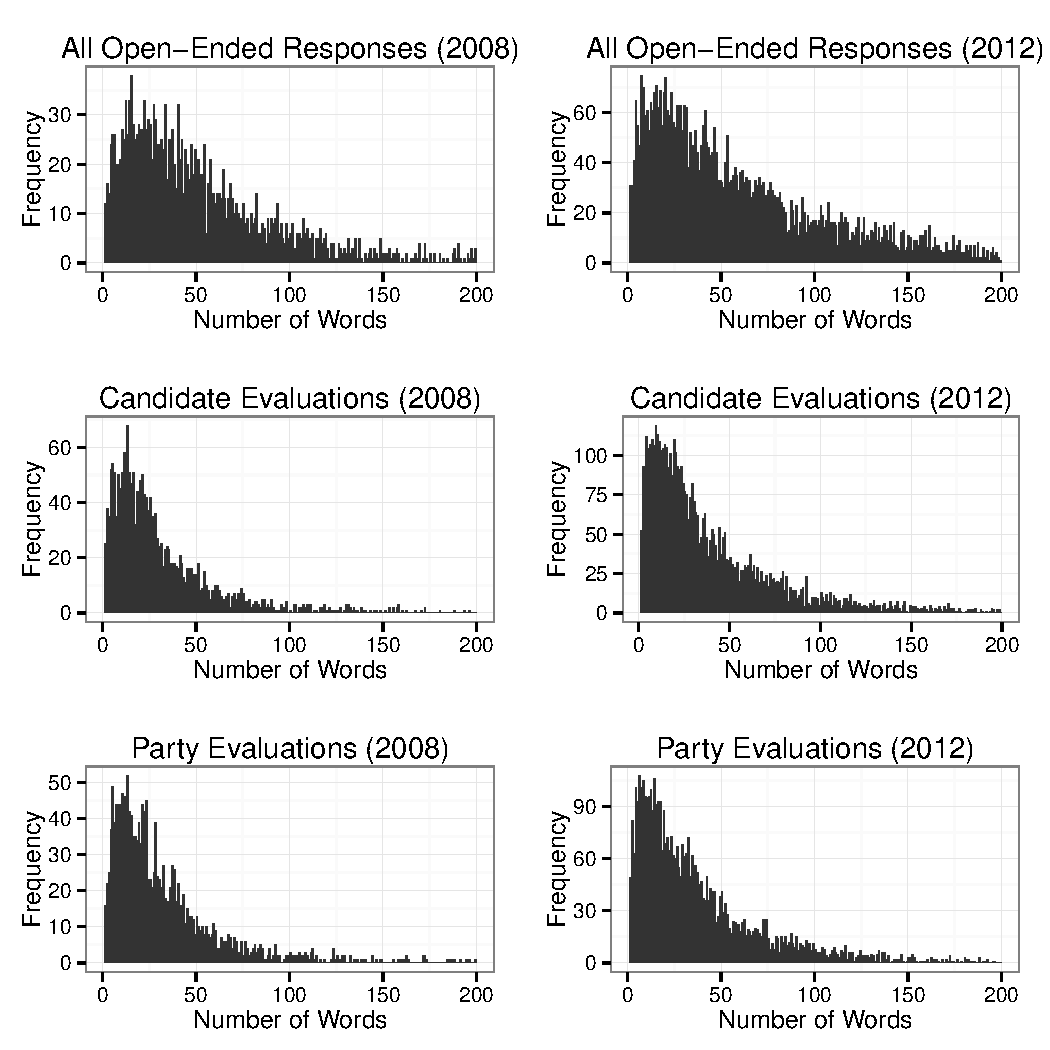
\includegraphics[height=.85\textheight]{../calc/fig/a0_num}
  \end{figure}
\end{frame}

\subsection{}
\begin{frame}%[allowframbreaks]
  \frametitle{Predicting Vote Choice using Moral Foundations}
  \begin{figure}[ht]\centering
    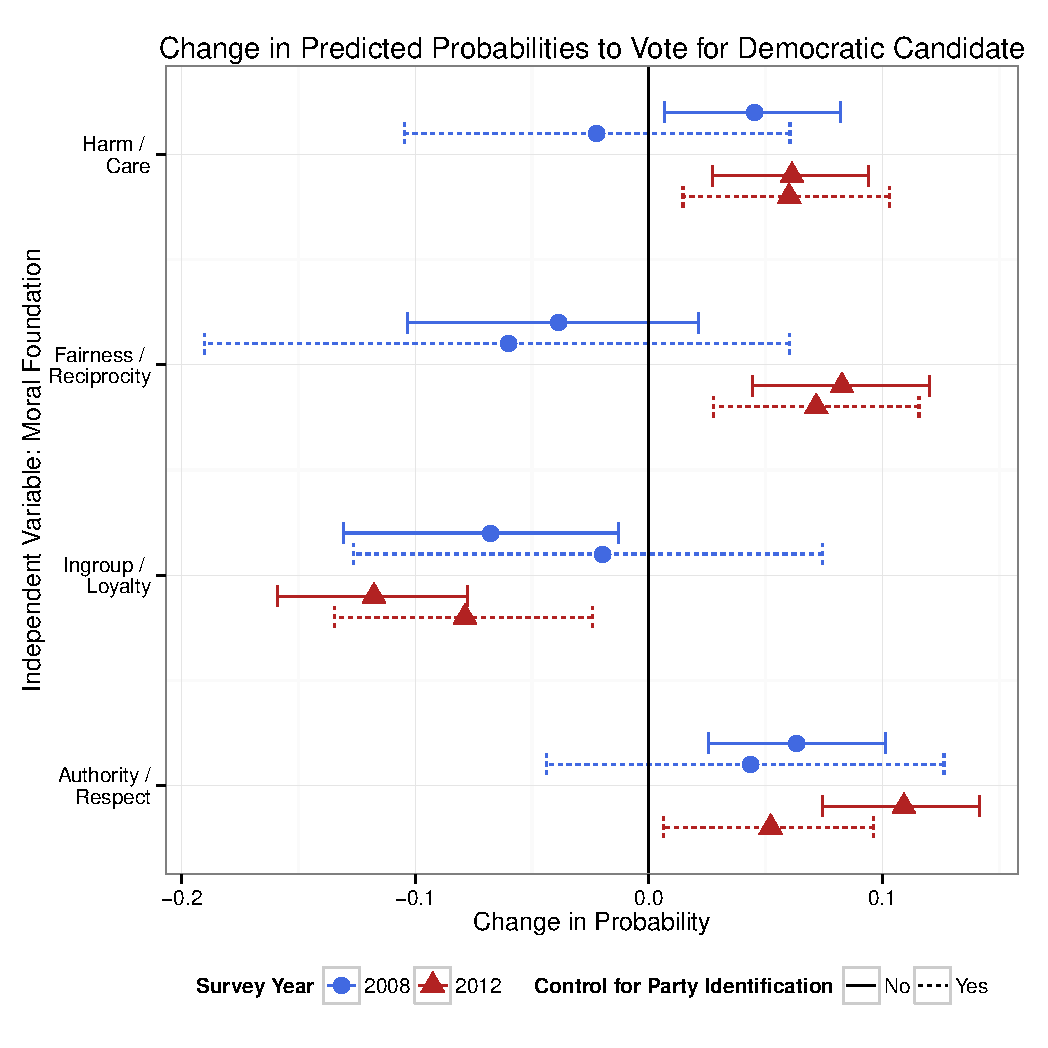
\includegraphics[height=.9\textheight]{../calc/fig/m2_vote}
  \end{figure}
\end{frame}

\subsection{}
\begin{frame}%[allowframbreaks]
\frametitle{Regression Discontinuity Design I}
  \begin{figure}[ht]\centering
    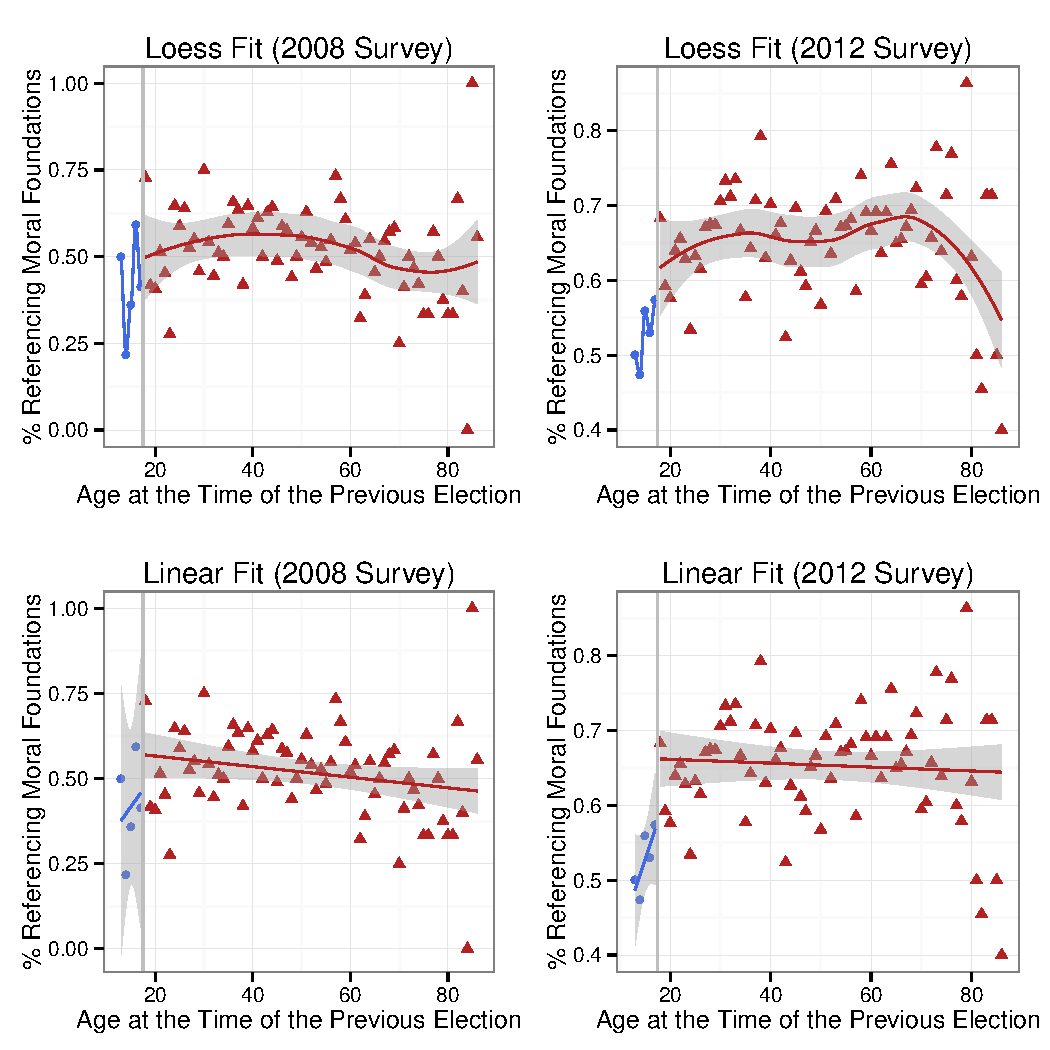
\includegraphics[height=.85\textheight]{../calc/fig/rd1_overview}
  \end{figure}
\end{frame}
\begin{frame}%[allowframbreaks]
\frametitle{Regression Discontinuity Design II}
\begin{scriptsize}
% latex table generated in R 3.1.3 by xtable 1.7-4 package
% Sun Apr 12 13:51:23 2015
\begin{table}[ht]
\centering
\begin{tabular}{lrrrrrrr}
  \hline
 & Bandwidth & Obs. & Est. & SE & Pr($>$$|$z$|$) & CI (low) & CI (high) \\ 
  \hline
LATE & 2.5302 & 166 & 0.5277 & 0.2016 & 0.0088 & 0.1327 & 0.9227 \\ 
  Half-BW & 1.2651 & 51 & 0.3135 & 0.1345 & 0.0198 & 0.0499 & 0.5771 \\ 
  Double-BW & 5.0604 & 268 & 0.1204 & 0.1333 & 0.3666 & -0.1409 & 0.3817 \\ 
   \hline
\end{tabular}
\caption{Regression Discontinuity Estimates Based on Age (2008)} 
\label{tab:rd2008y}
\end{table}

% latex table generated in R 3.2.2 by xtable 1.7-4 package
% Wed Sep 16 10:57:50 2015
\begin{table}[ht]
\centering
\begin{tabular}{lrrrrrrr}
  \hline
 & Bandwidth & Obs. & Est. & SE & Pr($>$$|$z$|$) & CI (low) & CI (high) \\ 
  \hline
LATE & 3.0998 & 415 & 0.1051 & 0.1075 & 0.3285 & 0.0960 & 0.8472 \\ 
  Half-BW & 1.5499 & 280 & 0.1123 & 0.1340 & 0.4020 & 0.0324 & 0.5475 \\ 
  Double-BW & 6.1997 & 672 & 0.0493 & 0.0840 & 0.5574 & -0.1696 & 0.3473 \\ 
   \hline
\end{tabular}
\caption{Regression Discontinuity Estimates Based on Age (2012)} 
\label{tab:rd2012y}
\end{table}

\end{scriptsize}
\end{frame}

\subsection{}
\begin{frame}
  \frametitle{References}
  \def\newblock{\hskip .11em plus .33em minus .07em}
  %\nocite{*}
  \begin{scriptsize}
    \bibliographystyle{apsr}
    \bibliography{/data/Copy/1-src/lit/Literature}
  \end{scriptsize}
\end{frame}

\end{document}